\documentclass[12pt,a4paper]{article}
\usepackage{ctex}
\usepackage{amsmath,amscd,amsbsy,amssymb,latexsym,url,bm,amsthm}
\usepackage{epsfig,graphicx,subfigure}
\usepackage{enumitem,balance}
\usepackage{wrapfig}
\usepackage{mathrsfs,euscript}
\usepackage[usenames]{xcolor}
\usepackage{hyperref}
\usepackage[vlined,ruled,linesnumbered]{algorithm2e}
\usepackage{array}
\hypersetup{colorlinks=true,linkcolor=black}

\newtheorem{theorem}{Theorem}
\newtheorem{lemma}[theorem]{Lemma}
\newtheorem{proposition}[theorem]{Proposition}
\newtheorem{corollary}[theorem]{Corollary}
\newtheorem{exercise}{Exercise}
\newtheorem*{solution}{Solution}
\newtheorem{definition}{Definition}
\theoremstyle{definition}

\renewcommand{\thefootnote}{\fnsymbol{footnote}}

\newcommand{\postscript}[2]
 {\setlength{\epsfxsize}{#2\hsize}
  \centerline{\epsfbox{#1}}}

\renewcommand{\baselinestretch}{1.0}

\setlength{\oddsidemargin}{-0.365in}
\setlength{\evensidemargin}{-0.365in}
\setlength{\topmargin}{-0.3in}
\setlength{\headheight}{0in}
\setlength{\headsep}{0in}
\setlength{\textheight}{10.1in}
\setlength{\textwidth}{7in}
\makeatletter \renewenvironment{proof}[1][Proof] {\par\pushQED{\qed}\normalfont\topsep6\p@\@plus6\p@\relax\trivlist\item[\hskip\labelsep\bfseries#1\@addpunct{.}]\ignorespaces}{\popQED\endtrivlist\@endpefalse} \makeatother
\makeatletter
\renewenvironment{solution}[1][Solution] {\par\pushQED{\qed}\normalfont\topsep6\p@\@plus6\p@\relax\trivlist\item[\hskip\labelsep\bfseries#1\@addpunct{.}]\ignorespaces}{\popQED\endtrivlist\@endpefalse} \makeatother

\begin{document}
\noindent

%========================================================================
\noindent\framebox[\linewidth]{\shortstack[c]{
\Large{\textbf{Lab10-Turing Machine}}\vspace{1mm}\\
CS214-Algorithm and Complexity, Xiaofeng Gao \& Lei Wang, Spring 2021.}}
\begin{center}
\footnotesize{\color{red}$*$ If there is any problem, please contact TA Yihao Xie. }

\footnotesize{\color{blue}$*$ Name:Zirui Liu  \quad Student ID:519021910343 \quad Email: L.prime@sjtu.edu.cn}
\end{center}

\begin{enumerate}
    \item Design a one-tape TM $M$ that computes the function $f(x, y) = \lfloor x/y \rfloor$, where $x$ and $y$ are positive integers $(x > y)$. The alphabet is $\{1, 0, \Box, \triangleright, \triangleleft\}$, and the inputs are $x$ "1"s, $\Box$ and $y$ "1"s. Below is the initial configuration for input $x=7$ and $y=3$. The result $z=f(x,y)$ should also be represented in the form of $z$ "1"s on the tape with pattern of $\rhd 111\cdots 111\lhd$, which is $\rhd 11\lhd$ for the example.
    
	\begin{center}
		\begin{tabular}{ll|c|c|c|c|c|c|c|c|c|c|c|c|c|c}
			& \multicolumn{14}{c}{Initial Configuration}\\[5pt]
			\cline{2-16}
			& & $\triangleright$ &  1  & 1 & 1 & 1 & 1 & 1 & 1 & $\Box$ & 1 & 1 & 1 & $ \triangleleft$ & \\
			\cline{2-16}
			\multicolumn{2}{c}{} & \multicolumn{1}{c}{$\uparrow$} & \multicolumn{11}{c}{}\\[-4px]
			\multicolumn{2}{c}{} & \multicolumn{1}{c}{$q_S$} & \multicolumn{11}{c}{}	
		\end{tabular}
	\end{center}

    \begin{enumerate}
	\item
	Please describe your design and then write the specifications of $M$ in the form like $\langle q_S, \triangleright \rangle \rightarrow \langle q_1, \triangleright,  R\rangle$. Explain the transition functions in detail.
	
	\item
	Please draw the state transition diagram.
	
	\item
	Show briefly and clearly the whole process from initial to final configurations for input $x = 7$ and $y = 3$. You may start like this:
	$$(q_s,\underline{\triangleright}  1  1  1  1  1  1  1  \Box 1  1  1   \triangleleft)
	\vdash (q_1,\triangleright  \underline{1}  1  1  1  1  1  1  \Box 1  1  1   \triangleleft)
	\vdash^* (q_1,\triangleright  1  1  1  1  1  1  1  \underline{\Box} 1  1  1   \triangleleft)
	\vdash (q_2,\triangleright  1  1  1  1  1  1  1  \Box \underline{1}  1  1   \triangleleft)$$
	
	\par{\color{blue}(Note that for simplicity, we write $(q_1,\triangleright  \underline{1}  1  1  1  1  1  1  \Box 1  1  1   \triangleleft)\vdash^* (q_1,\triangleright  1  1  1  1  1  1  1  \underline{\Box} 1  1  1   \triangleleft)$ if the corresponding transaction repeats on multiple inputs with the same state.)}
	
\end{enumerate}

    \begin{solution}
    (a):\\
    \begin{equation*}
        \begin{aligned}
        & \langle q_s, \triangleright \rangle  \rightarrow  \langle q_1, \triangleright, R\rangle
        & \langle q_1, 0 \rangle  \rightarrow  \langle q_1, 0, R\rangle \\
        & \langle q_1, 1 \rangle  \rightarrow  \langle q_1, 1, R\rangle
        & \langle q_1, \Box \rangle  \rightarrow  \langle q_1, \Box, R\rangle \\
        & \langle q_1, \triangleright \rangle  \rightarrow  \langle q_1, \triangleright, R\rangle
        & \langle q_1, \triangleleft \rangle  \rightarrow  \langle q_2, \triangleleft, R\rangle   \\
        & \langle q_2, 0 \rangle  \rightarrow  \langle q_2, 0, L\rangle
        & \langle q_2, 1 \rangle  \rightarrow  \langle q_3, 0, L\rangle \\
        & \langle q_2, \Box \rangle  \rightarrow  \langle q_7, \Box, R\rangle 
        & \langle q_7, 0 \rangle  \rightarrow  \langle q_7, 1, R\rangle \\
        & \langle q_7, 1 \rangle  \rightarrow  \langle q_7, 1, R\rangle
        & \langle q_7, \triangleleft \rangle  \rightarrow  \langle q_5, \triangleleft, L\rangle  \\
        & \langle q_3, 1 \rangle  \rightarrow  \langle q_3, 1, L\rangle
        & \langle q_3, \Box \rangle  \rightarrow  \langle q_4, \Box, L\rangle \\
        & \langle q_4, 0 \rangle  \rightarrow  \langle q_4, 0, L\rangle 
        & \langle q_4, 1 \rangle  \rightarrow  \langle q_1, 0, R\rangle \\
        & \langle q_4, \triangleright \rangle  \rightarrow  \langle q_8, \triangleleft, R\rangle
        & \langle q_5, 0 \rangle  \rightarrow  \langle q_5, 0, L\rangle  \\
        & \langle q_5, 1 \rangle  \rightarrow  \langle q_5, 1, L\rangle
        & \langle q_5, \Box \rangle  \rightarrow  \langle q_5, \Box, L\rangle \\
        & \langle q_5, \triangleright \rangle  \rightarrow  \langle q_6, \triangleright, L\rangle 
        & \langle q_6, 0 \rangle  \rightarrow  \langle q_6, 0, L\rangle \\
        & \langle q_6, 1 \rangle  \rightarrow  \langle q_6, 1, L\rangle
        & \langle q_6, \Box \rangle  \rightarrow  \langle q_1, 1, R\rangle  \\
        & \langle q_8, 0 \rangle  \rightarrow  \langle q_8, \Box, R\rangle
        & \langle q_8, 1 \rangle  \rightarrow  \langle q_8, \Box, R\rangle \\
        & \langle q_8, \Box \rangle  \rightarrow  \langle q_8, \Box, R\rangle 
        & \langle q_8, \triangleleft \rangle  \rightarrow  \langle q_9, \Box, L\rangle \\
        & \langle q_9, \Box \rangle  \rightarrow  \langle q_9, \Box, L\rangle
        & \langle q_9, \triangleleft \rangle  \rightarrow  \langle q_{10}, \triangleleft, L\rangle  \\
        & \langle q_{10}, 1 \rangle  \rightarrow  \langle q_{10}, 1, L\rangle
        & \langle q_{10}, \Box \rangle  \rightarrow  \langle q_e, \triangleright, L\rangle  \\
        
        
        
        
        
        
        
        
        \end{aligned}
    \end{equation*}
    
    
    
    (b):\\
    		\begin{figure}[!htbp]
			\centering
			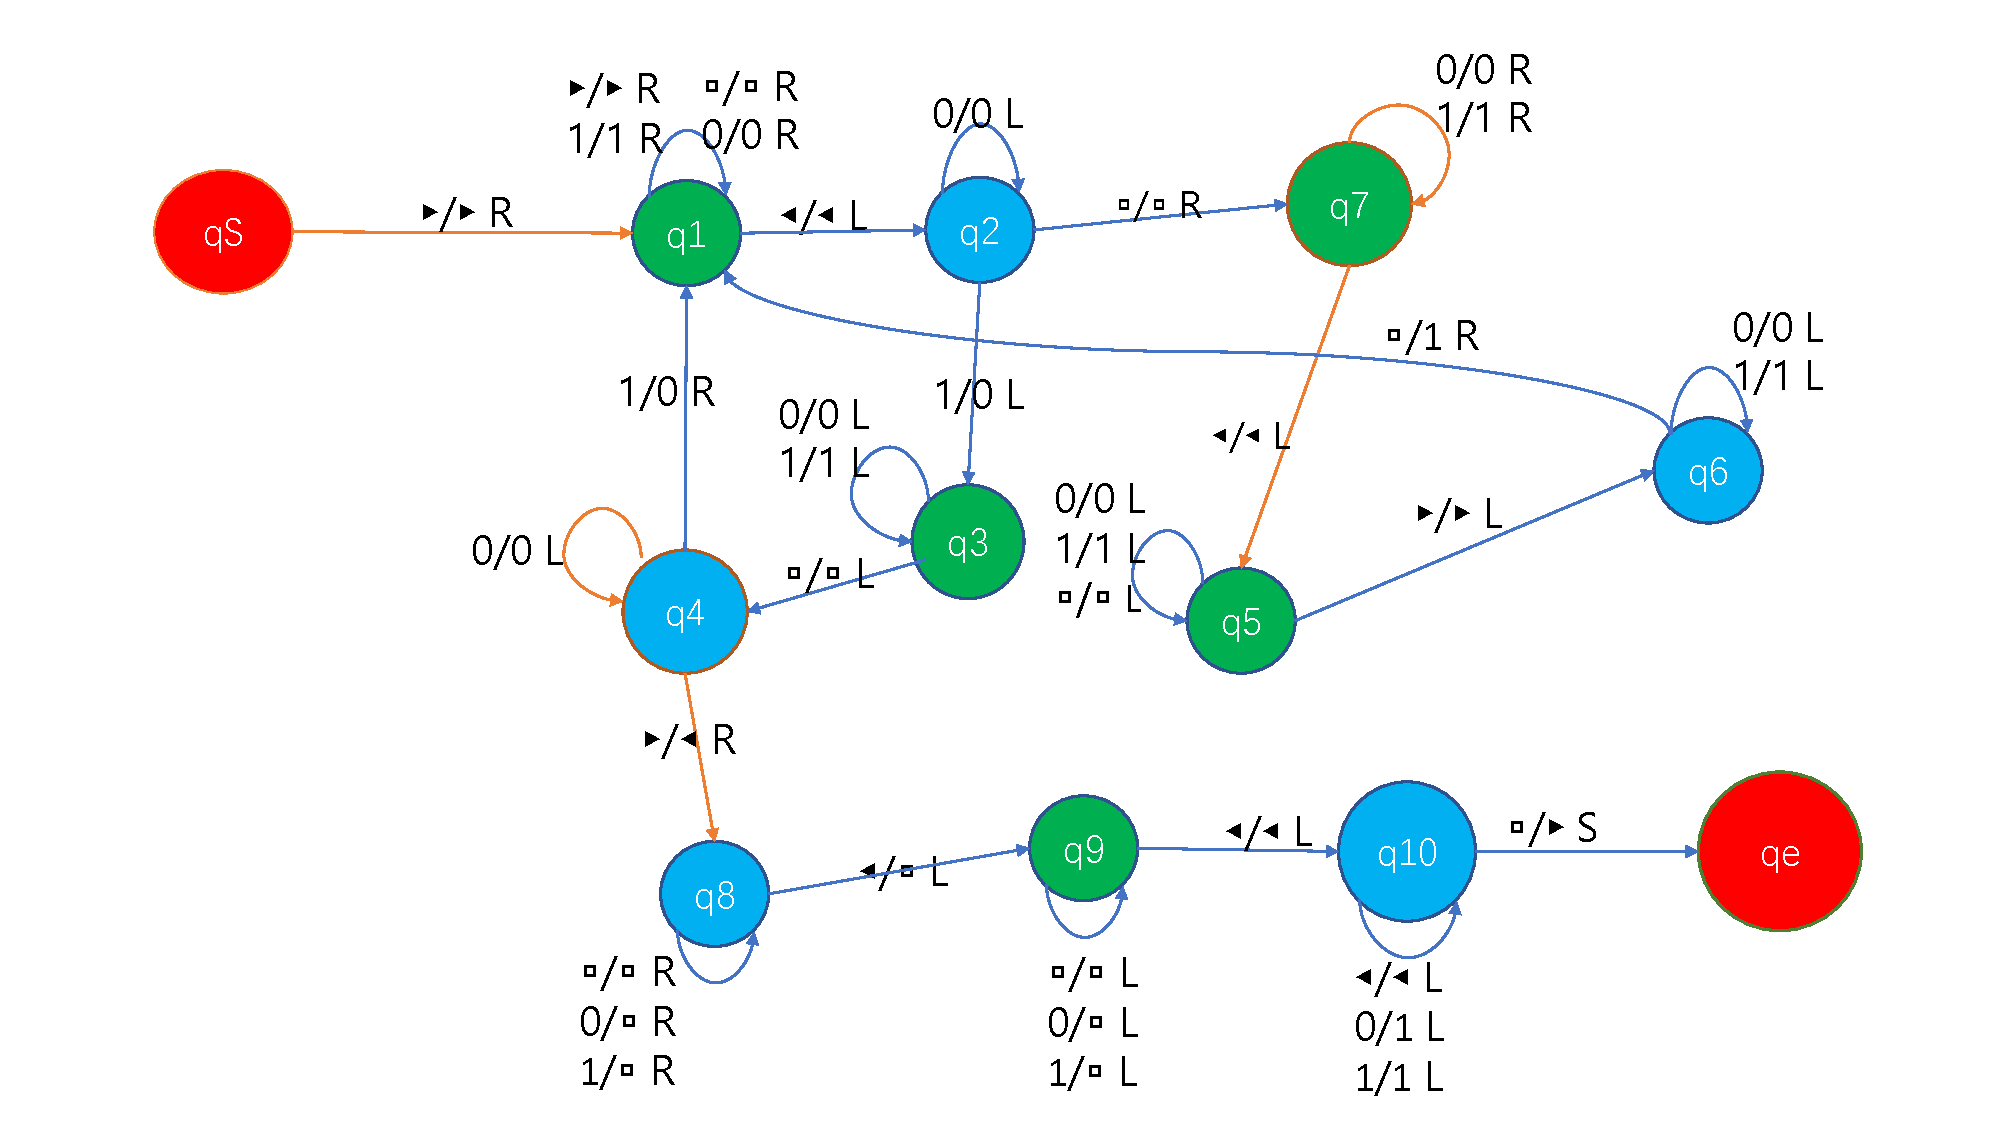
\includegraphics[width=0.9\textwidth]{pic.pdf}
			\caption{Turing Machine}
			\label{ }
		\end{figure}
    
    
    (c):\\
    \begin{equation*}
        \begin{aligned}
    &(q_s,\underline{\triangleright}  1  1  1  1  1  1  1  \Box 1  1  1   \triangleleft)
    &\vdash (q_1,\triangleright  \underline{1}  1  1  1  1  1  1  \Box 1  1  1   \triangleleft)
    &\vdash (q_1,\triangleright  1  1  1  1  1  1  1  \underline{\Box} 1  1  1   \triangleleft)
    \\
    &\vdash (q_1,\triangleright  1  1  1  1  1  1  1  \Box \underline{1}  1  1   \triangleleft)
    &\vdash (q_1,\triangleright  1  1  1  1  1  1  1  \Box 1  1  1   \underline\triangleleft)
    &\vdash (q_2,\triangleright  1  1  1  1  1  1  1  \Box 1  1  \underline1   \triangleleft)
    \\
    &\vdash (q_3,\triangleright  1  1  1  1  1  1  1  \Box 1  \underline1  0   \triangleleft)
    &\vdash (q_3,\triangleright  1  1  1  1  1  1  1  \underline\Box 1  1  0   \triangleleft)
    &\vdash (q_4,\triangleright  1  1  1  1  1  1  \underline1  \Box 1  1  0   \triangleleft)
\\
    &\vdash (q_1,\triangleright  1  1  1  1  1  1  0  \underline\Box 1  1  0   \triangleleft)
    &\vdash (q_1,\triangleright  1  1  1  1  1  1  0  \Box 1  1  \underline0   \triangleleft)
    &\vdash (q_1,\triangleright  1  1  1  1  1  1  0  \Box 1  1  0   \underline\triangleleft)
\\
    &\vdash (q_2,\triangleright  1  1  1  1  1  1  0  \Box 1  1  \underline0   \triangleleft)
    &\vdash (q_2,\triangleright  1  1  1  1  1  1  0  \Box 1  \underline1 0  \triangleleft)
    &\vdash (q_3,\triangleright  1  1  1  1  1  1  0  \Box \underline{1}  0  0   \triangleleft)
\\
    &\vdash (q_3,\triangleright  1  1  1  1  1  1  0  \underline\Box 1  0  0   \triangleleft)
    &\vdash (q_4,\triangleright  1  1  1  1  1  1  \underline0  \Box 1 0 0   \triangleleft)
    &\vdash (q_4,\triangleright  1  1  1  1  1  \underline1  0  \Box 1 0 0   \triangleleft)
\\
    &\vdash (q_1,\triangleright  1  1  1  1  1  0  \underline0  \Box 1  0  0   \triangleleft)
    &\vdash (q_1,\triangleright  1  1  1  1  1  0  0  \Box 1  0  0   \underline\triangleleft)
    &\vdash (q_2,\triangleright  1  1  1  1  1  0  0  \Box 1  0  \underline0   \triangleleft)
\\
    &\vdash (q_2,\triangleright  1  1  1  1  1  0  0  \Box \underline{1}  0  0   \triangleleft)
    &\vdash (q_3,\triangleright  1  1  1  1  1  0  0  \underline\Box 0  0  0   \triangleleft)
    &\vdash (q_4,\triangleright  1  1  1  1  1  0  \underline0  \Box 0  0  0   \triangleleft)
\\
    &\vdash (q_4,\triangleright  1  1  1  1  \underline1  0  0  \Box 0  0  0   \triangleleft)
    &\vdash (q_1,\triangleright  1  1  1  1  0  \underline0  0  \Box 0  0  0   \triangleleft)
    &\vdash (q_1,\triangleright  1  1  1  1  0  0  0  \Box 0  0  0  \underline\triangleleft)
\\
    &\vdash (q_2,\triangleright  1  1  1  1  0  0  0  \Box 0  0 \underline0  \triangleleft)
    &\vdash (q_2,\triangleright  1  1  1  1  0  0  0  \underline\Box 0  0 0  \triangleleft)
    &\vdash (q_7,\triangleright  1  1  1  1  0  0  0  \Box \underline0  0 0  \triangleleft)
\\
    &\vdash (q_7,\triangleright  1  1  1  1  0  0  0  \Box 1 \underline0   0  \triangleleft)
    &\vdash (q_7,\triangleright  1  1  1  1  0  0  0  \Box 1 1   \underline0  \triangleleft)
    &\vdash (q_7,\triangleright  1  1  1  1  0  0  0  \Box 1 1 1 \underline  \triangleleft)
\\
    &\vdash (q_5,\triangleright  1  1  1  1  0  0  0  \Box 1 1 \underline1 \triangleleft)
    &\vdash (q_5,\triangleright  1  1  1  1  0  0  0  \underline\Box 1 1 1 \triangleleft)
    &\vdash (q_5,\Box \Box \Box \underline\triangleright  1  1  1  1  0  0  0  \Box 1 1 1 \triangleleft)
\\
    &\vdash (q_6,\Box \Box \underline\Box \triangleright  1  1  1  1  0  0  0  \Box 1 1 1 \triangleleft)
    &\vdash (q_1,\Box \Box 1 \underline\triangleright  1  1  1  1  0  0  0  \Box 1 1 1 \triangleleft)
    &\vdash (q_1,\Box \Box 1 \triangleright  1  1  1  1  0  0  0  \Box 1 1 1 \underline\triangleleft)
\\
    &\vdash (q_2,\Box \Box 1 \triangleright  1  1  1  1  0  0  0  \Box 1 1 \underline1 \triangleleft)
    &\vdash (q_3,\Box \Box 1 \triangleright  1  1  1  1  0  0  0  \Box 1 \underline1 0 \triangleleft)
    &\vdash (q_3,\Box \Box 1 \triangleright  1  1  1  1  0  0  0  \underline\Box 1 1 0 \triangleleft)
\\
    &\vdash (q_4,\Box \Box 1 \triangleright  1  1  1  1  0  0  \underline0  \Box 1 1 0 \triangleleft)
    &\vdash (q_4,\Box \Box 1 \triangleright  1  1  1  \underline1  0  0  0  \Box 1 1 0 \triangleleft)
    &\vdash (q_1,\Box \Box 1 \triangleright  1  1  1  0  \underline0  0  0  \Box 1 1 0 \triangleleft)
\\
    &\vdash (q_1,\Box \Box 1 \triangleright  1  1  1  0  0  0  0  \Box 1 1 0 \underline\triangleleft)
    &\vdash (q_2,\Box \Box 1 \triangleright  1  1  1  0  0  0  0  \Box 1 1 \underline0 \triangleleft)
    &\vdash (q_2,\Box \Box 1 \triangleright  1  1  1  0  0  0  0  \Box 1 \underline1 0 \triangleleft)
\\
    &\vdash (q_3,\Box \Box 1 \triangleright  1  1  1  0  0  0  0  \Box \underline1 0 0 \triangleleft)
    &\vdash (q_3,\Box \Box 1 \triangleright  1  1  1  0  0  0  0  \underline\Box 1 0 0 \triangleleft)
    &\vdash (q_4,\Box \Box 1 \triangleright  1  1  1  0  0  0  \underline0  \Box 1 0 0 \triangleleft)
\\
    &\vdash (q_4,\Box \Box 1 \triangleright  1  1  \underline1  0  0  0  0  \Box 1 0 0 \triangleleft)
    &\vdash (q_1,\Box \Box 1 \triangleright  1  1  0  \underline0  0  0  0  \Box 1 0 0 \triangleleft)
    &\vdash (q_1,\Box \Box 1 \triangleright  1  1  0  0  0  0  0  \Box 1 0 0 \underline\triangleleft)
\\
    &\vdash (q_2,\Box \Box 1 \triangleright  1  1  0  0  0  0  0  \Box 1 0 \underline0  \triangleleft)
    &\vdash (q_2,\Box \Box 1 \triangleright  1  1  0  0  0  0  0  \Box \underline1 0 0  \triangleleft)
    &\vdash (q_3,\Box \Box 1 \triangleright  1  1  0  0  0  0  0  \underline\Box 0 0 0  \triangleleft)
\\
    &\vdash (q_4,\Box \Box 1 \triangleright  1  1  0  0  0  0  \underline0  \Box 0 0 0  \triangleleft)
    &\vdash (q_4,\Box \Box 1 \triangleright  1  \underline1  0  0  0  0  0  \Box 0 0 0  \triangleleft)
    &\vdash (q_1,\Box \Box 1 \triangleright  1  0  \underline0  0  0  0  0  \Box 0 0 0  \triangleleft)
\\
    &\vdash (q_1,\Box \Box 1 \triangleright  1  0  0  0  0  0  0  \Box 0 0 0  \underline\triangleleft)
    &\vdash (q_2,\Box \Box 1 \triangleright  1  0  0  0  0  0  0  \Box 0 0 \underline0 \triangleleft)
    &\vdash (q_2,\Box \Box 1 \triangleright  1  0  0  0  0  0  0  \underline\Box 0 0 0 \triangleleft)
\\
    &\vdash (q_7,\Box \Box 1 \triangleright  1  0  0  0  0  0  0  \Box \underline0 0 0 \triangleleft)
    &\vdash (q_7,\Box \Box 1 \triangleright  1  0  0  0  0  0  0  \Box 1 1 1 \underline\triangleleft)
    &\vdash (q_5,\Box \Box 1 \triangleright  1  0  0  0  0  0  0  \Box 1 1 \underline1 \triangleleft)
\\
    &\vdash (q_5,\Box \Box 1 \underline\triangleright  1  0  0  0  0  0  0  \Box 1 1 1 \triangleleft)
    &\vdash (q_6,\Box \Box 1 \underline\triangleright  1  0  0  0  0  0  0  \Box 1 1 1 \triangleleft)
    &\vdash (q_6,\Box \underline\Box 1 \triangleright  1  0  0  0  0  0  0  \Box 1 1 1 \triangleleft)
\\
    &\vdash (q_1,\Box 1 \underline1 \triangleright  1  0  0  0  0  0  0  \Box 1 1 1 \triangleleft)
    &\vdash (q_1,\Box 1 1 \triangleright  1  0  0  0  0  0  0  \Box 1 1 1 \underline\triangleleft)
    &\vdash (q_2,\Box 1 1 \triangleright  1  0  0  0  0  0  0  \Box 1 1 \underline1 \triangleleft)
\\
    &\vdash (q_3,\Box 1 1 \triangleright  1  0  0  0  0  0  0  \Box 1 \underline1 0 \triangleleft)
    &\vdash (q_3,\Box 1 1 \triangleright  1  0  0  0  0  0  0  \underline\Box 1 1 0 \triangleleft)
    &\vdash (q_4,\Box 1 1 \triangleright  1  0  0  0  0  0  \underline0  \Box 1 1 0 \triangleleft)
\\
    &\vdash (q_4,\Box 1 1 \triangleright  \underline1  0  0  0  0  0  0  \Box 1 1 0 \triangleleft)
    &\vdash (q_1,\Box 1 1 \triangleright  0  \underline0  0  0  0  0  0  \Box 1 1 0 \triangleleft)
    &\vdash (q_1,\Box 1 1 \triangleright  0  0  0  0  0  0  0  \Box 1 1 0 \underline\triangleleft)
\\
    &\vdash (q_2,\Box 1 1 \triangleright  0  0  0  0  0  0  0  \Box 1 1 \underline0 \triangleleft)
    &\vdash (q_2,\Box 1 1 \triangleright  0  0  0  0  0  0  0  \Box 1 \underline1 0 \triangleleft)
    &\vdash (q_3,\Box 1 1 \triangleright  0  0  0  0  0  0  0  \Box \underline1 0 0 \triangleleft)
\\
    &\vdash (q_3,\Box 1 1 \triangleright  0  0  0  0  0  0  0  \underline\Box 1 0 0 \triangleleft)
    &\vdash (q_4,\Box 1 1 \triangleright  0  0  0  0  0  0  \underline0  \Box 1 0 0 \triangleleft)
    &\vdash (q_4,\Box 1 1 \underline\triangleright  0  0  0  0  0  0  0  \Box 1 0 0 \triangleleft)
\\
    &\vdash (q_8,\Box 1 1 \triangleleft \underline0  0  0  0  0  0  0  \Box 1 0 0 \triangleleft)
    &\vdash (q_8,\Box 1 1 \triangleleft \Box  \underline0  0  0  0  0  0  \Box 1 0 0 \triangleleft)
    &\vdash (q_8,\Box 1 1 \triangleleft \Box  \Box  \Box  \Box  \Box  \Box  \Box  \underline\Box 1 0 0 \triangleleft)
\\
    &\vdash (q_8,\Box 1 1 \triangleleft \Box  \Box  \Box  \Box  \Box  \Box  \Box  \Box \Box \Box \Box \underline\triangleleft)
    &\vdash (q_9,\Box 1 1 \triangleleft \Box  \Box  \Box  \Box  \Box  \Box  \Box  \Box \Box \Box \underline\Box \Box)
    &\vdash (q_9,\Box 1 1 \underline\triangleleft)
\\
    &\vdash (q_{10},\Box 1 \underline1 \triangleleft)
    &\vdash (q_{10},\underline\Box 1 1 \triangleleft)
    &\vdash (q_{e},\underline\triangleright 1 1 \triangleleft)
    
    
    
    
        \end{aligned}
    \end{equation*}

    
    \end{solution}
    

    \item 
    Given the alphabet $\{1, 0, \Box, \triangleright, \triangleleft\}$, design a time efficient 3-tape TM $M$ to compute $f:\{0,1\}^*\rightarrow\{0,1\}$ which verifies whether the number of 0 and the number of 1 are the same in an input consisting of only 0's and 1's. $M$ should output 1 if the numbers are the same, and 0 otherwise. For eample, for the input tape $\triangleright 001101\triangleleft$, $M$ should output 1
    
    \begin{enumerate}
	    \item
	    Please describe your design and then write the specifications of $M$ in the form like $\langle q_S, \triangleright, \triangleright, \triangleright \rangle \rightarrow \langle q_1, \triangleright,\triangleright,  R, R, S \rangle$. Explain the transition functions in detail.
	    
	    \item 
	    Show the time complexity for one-tape TM $M'$ to compute the same function $f$ with $n$ symbols in the input and give a brief description of such $M'$ .
	
	\end{enumerate}
    

	\begin{solution}
		(a):\\
		
	\textbf{Begin To Copy}
    \begin{equation*}
    \begin{aligned}
    &\langle q_s, \triangleright, \Box, \Box\rangle \rightarrow \langle q_1,    \triangleright, \Box, R, R, S\rangle \\
    &\langle q_1, 0, \Box, \Box\rangle \rightarrow \langle q_1, 0, \Box, R, S, S\rangle \\
    &\langle q_1, 1, \Box, \Box\rangle \rightarrow \langle q_1, \Box, 1, R, S, R\rangle \\
    &\langle q_1, \triangleleft, \Box, \Box\rangle \rightarrow \langle q_2, \triangleleft, \Box, S, L, L\rangle \\
    \end{aligned}
    \end{equation*}

	\textbf{Check Equal Or Not}

    \begin{equation*}
    \begin{aligned}
    &\langle q_2, \triangleleft, 0, 1\rangle \rightarrow \langle q_2, 0, \Box, S, L, L\rangle \\
    &\langle q_2, \triangleleft, 0, \Box\rangle \rightarrow \langle q_e, 0, 0, S, S, S\rangle \\
    &\langle q_2, \triangleleft, \triangleright, \Box\rangle \rightarrow \langle q_e, \triangleright, 1, S, S, S\rangle \\
    \end{aligned}
    \end{equation*}

	\textbf{Output}

    \begin{equation*}
    \begin{aligned}
    &\langle q_2, \triangleleft, \triangleright, 1\rangle \rightarrow \langle q_3, \triangleright, \Box, S, S, L\rangle \\
    &\langle q_3, \triangleleft, \triangleright, 1\rangle \rightarrow \langle q_3, \triangleright, \Box, S, S, L\rangle \\
    &\langle q_3, \triangleleft, \triangleright, \Box\rangle \rightarrow \langle q_e, \triangleright, 0, S, S, S\rangle \\
    \end{aligned}
    \end{equation*}

	(b):\\
	
	We know that if $f:\{0,1\}^*\rightarrow \{0, 1\}^*$ is computable in time $T(n)$ by using $k$ tapes, then it is computable in time $5kT(n)^2$ using one tape TM. In problem $a$, we have $k=3$ and $T(n)=O(n)$, so we can know that the time complexity for one tape TM is $O(n^2)$.

	For such $M'$, we thought that it is proper to match every $0$ and $1$. The head should scan round and round and every time the head
	matches one $0$ and one $1$, it should turn both of them into $\Box$. If the head can't match such one $0$ and one $1$ (when the tape is not empty)
	then we knew it won't match, so we will output $0$. On the other hand, it would output $1$. The TM will go through at most $n$ rounds, and each round costs $n$ movements,
	For the fact that one tape TM has nearly the same complexity as multi tape TM, so in conclusion, the time complexity is $O(n^2)$.

\end{solution}
    
	
	\item Define the corresponding decision or search problem of the following problems and give the "certificate" and "certifier" for each decision problem provided in the subquestions or defined by yourself.
	
	\begin{enumerate}
	    \item
	    \textit{3-Dimensional Matching.}  Given disjoint sets $X,Y,Z$ all with the size of $n$, and a set $M \subseteq X\times Y\times Z$.  Is there a subset $M'$ of $M$ of size $n$ where no two elements of $M'$ agree in any coordinate?
	    
	    \item 
	    \textit{Travelling Salesman Problem.} Given a list of cities and the distances between each pair of cities, find the shortest possible route that visits each city exactly once and returns to the origin city.
	    
	    \item
	    \textit{Job Sequencing.} Given a set of unit-time jobs, each of which has an integer deadline and a nonnegative penalty for missing the deadline. Does there exist a job sequence that has a total penalty $w\leqslant k$?
	    
	\end{enumerate}
	
	\begin{solution}
    (a):\\
    \textbf{Certificate:} 
    Give permutation for all the three dimension tuple. \\
    
    \textbf{Certifier:}
    Check for all the permutation, does it satisfy the condition of no two elements having the same coordinate.
    
    (b):\\
    \textbf{Certificate:} 
    A permutation of the $n$ nodes.
    
    \textbf{Certifier:}
    Check that the permutation contains each node in $V$ exactly once(except the start point, which also being the end point,would be contained twice) , and that there is an edge between each pair of adjacent nodes in the permutation to form a circle.
    
    (c):\\
    \textbf{Certificate:} 
    We can apply the greedy algorithm. First we sort all the jobs in decreasing order of their penalties so that minimum of penalties will be charged.
    
    \textbf{Certifier:}
    Using contradiction, it is easy to prove the optimality of the greedy algorithm.
    
    
    \end{solution}
	
	
\end{enumerate}

\textbf{Remark:} Please include your .pdf, .tex files for uploading with standard file names.
\newpage


%========================================================================
\end{document}